\section{Methodology}\label{sec:methodology}

\subsection{Dataset}

Our dataset is derived from the publically available Face Research Lab London~\cite{frll} (FRLL) set, comprising 102 frontal ICAO-compliant facial images. Each image was encoded using four printer-proof steganographic methods, described ahead, each applied at nine different intensity levels, yielding a total of 3,672 distorted images.

The dataset was partitioned into four subsets, as follows:

\begin{itemize}
    \item MOS set (15 identities, 540 images): a core set of demographically diverse subjects, shown in Fig.~\ref{fig:mos_set}, with subjective MOS annotations. It is split into:
    \begin{itemize}
        \item MOS train set (12 identities): used to train the FR fusion model, regressing FR-IQA metrics to human MOS.\@
        \item MOS test set (3 identities): held out from the framework and used only for final evaluation.
    \end{itemize}
    \item Pseudo-MOS set (87 identities, 3,132 images): no subjective scores were collected for these images. Pseudo-MOS are generated for this set using the trained fusion model.
    \item NR train set: includes both the MOS train set and the pseudo-MOS set. It is used to train the NR regressor.
\end{itemize}

\begin{figure}
    \centering
    \begin{minipage}[t]{0.76\textwidth}
        \centering
        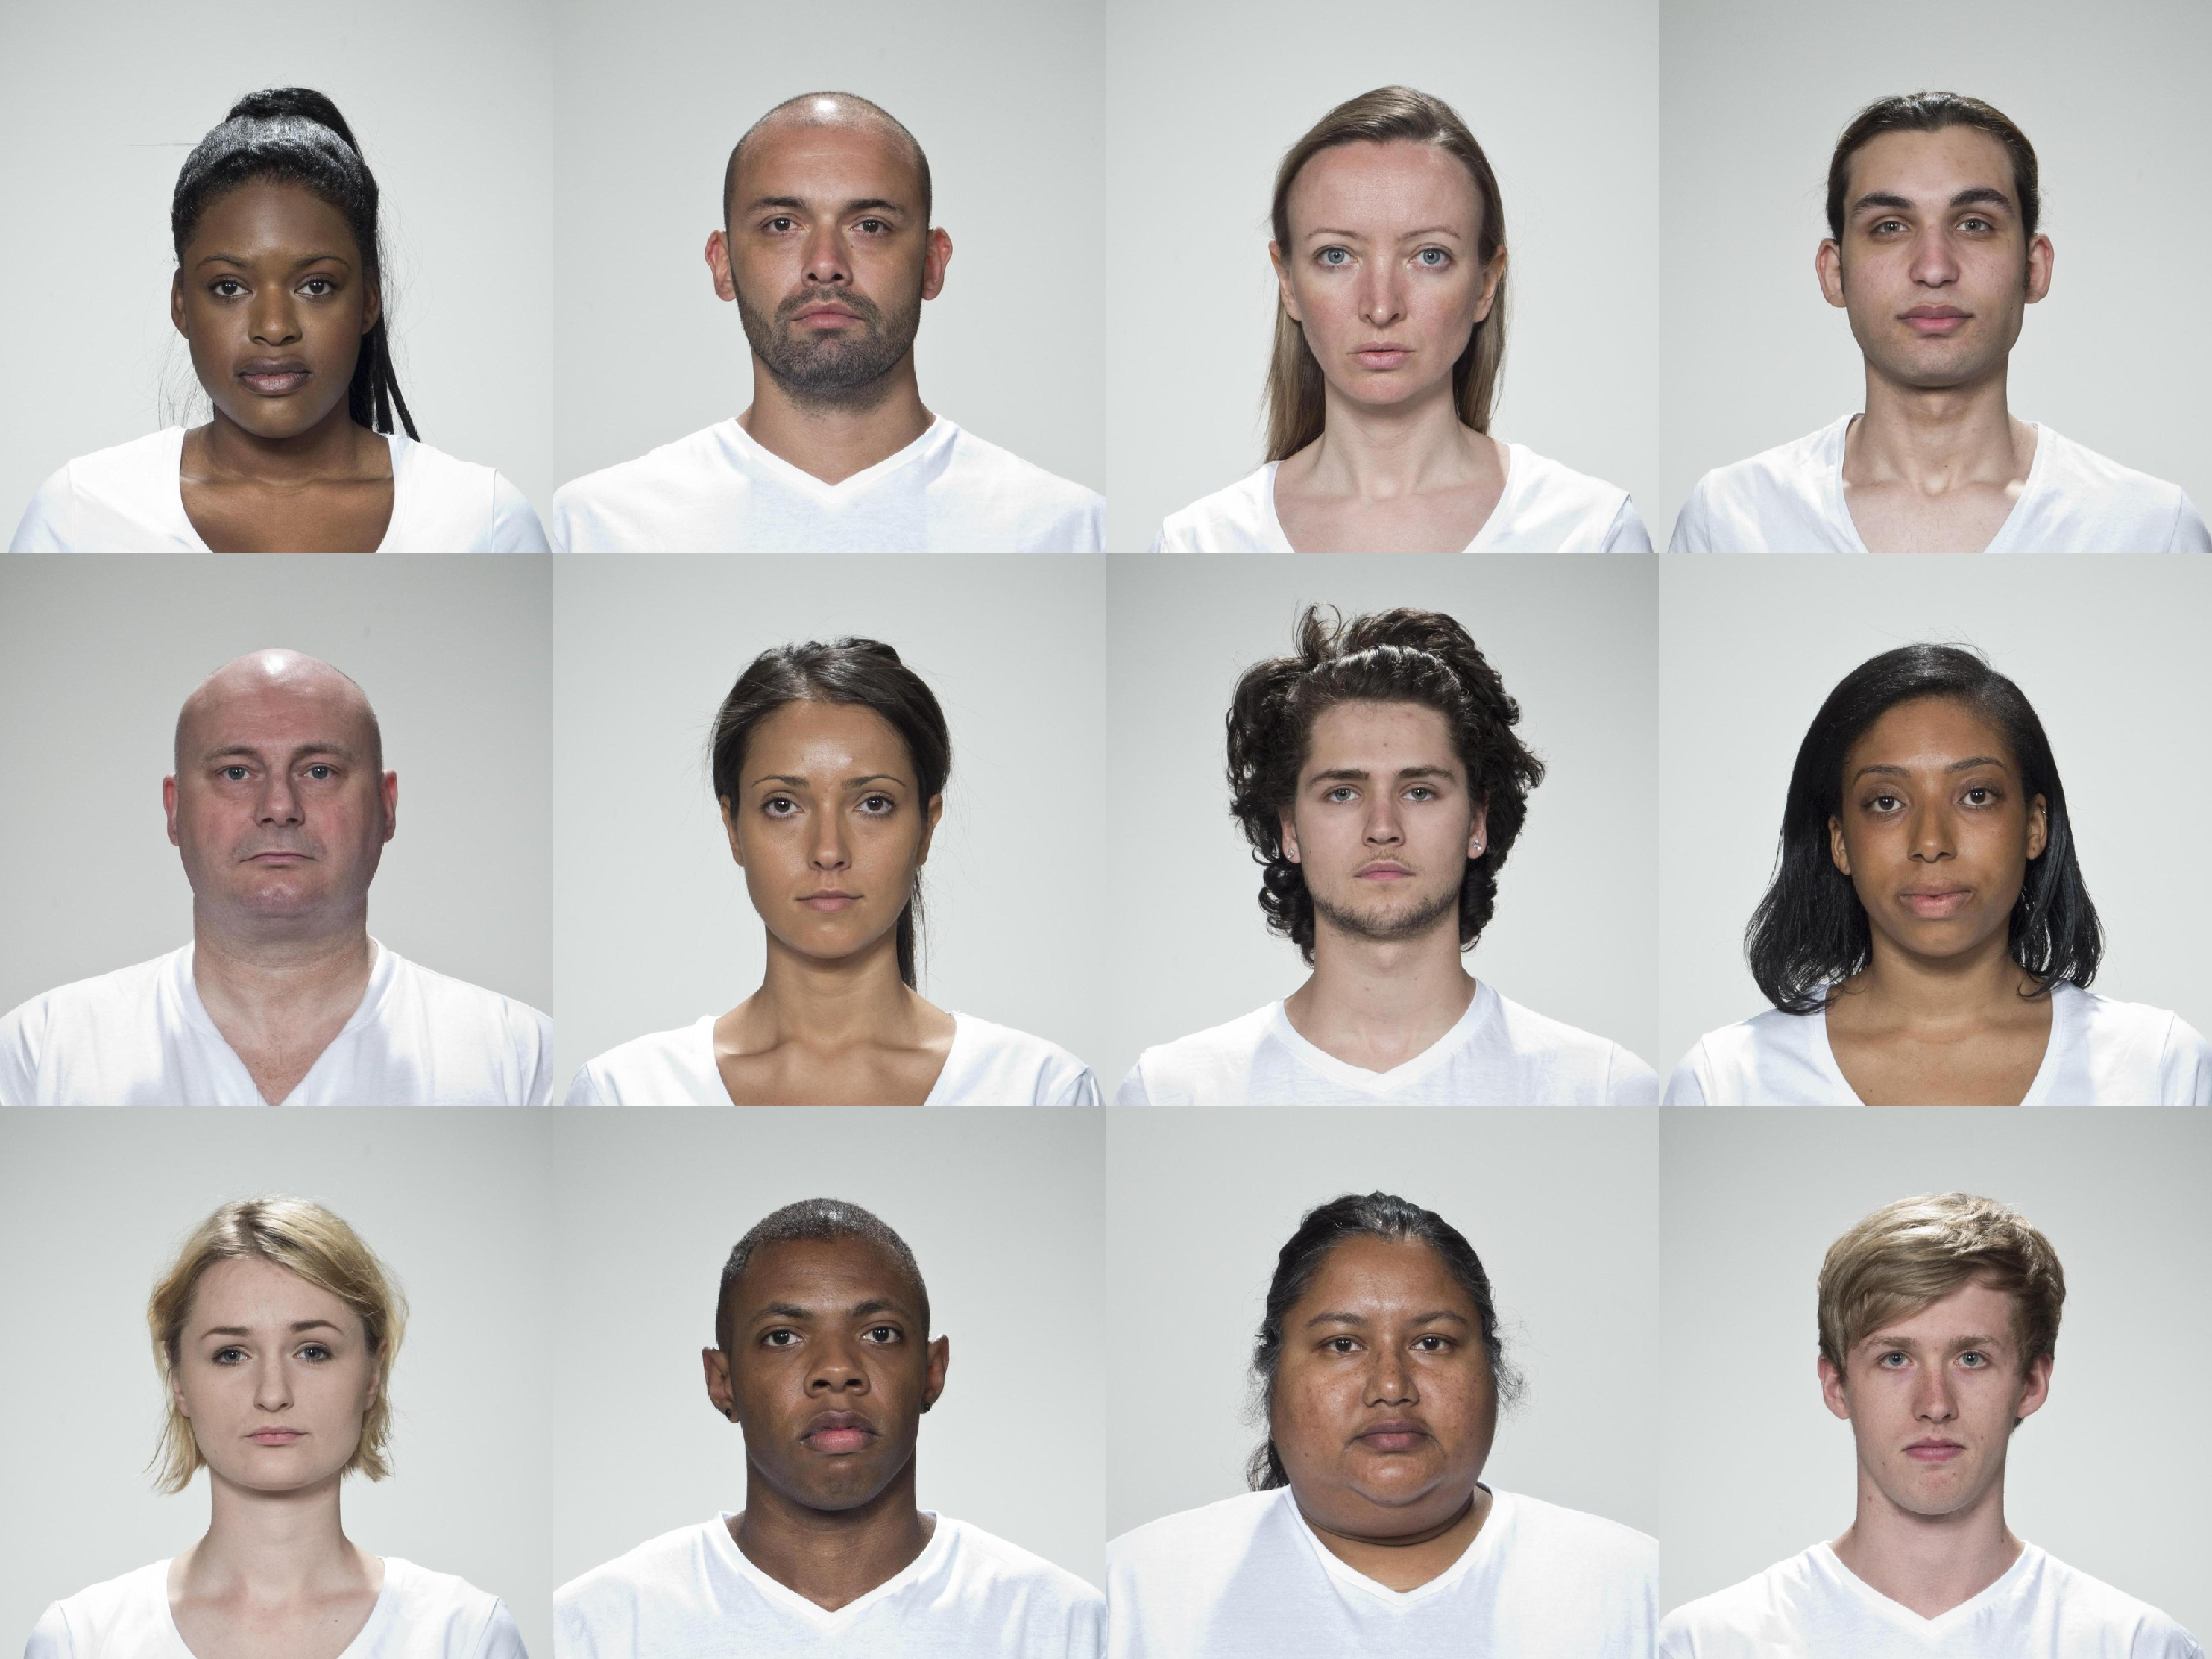
\includegraphics[width=\textwidth]{images/mos_train_set.pdf}\\
        \textbf{(a)} MOS train set % chktex 10
    \end{minipage}
    \hfill
    \begin{minipage}[t]{0.19\textwidth}
        \centering
        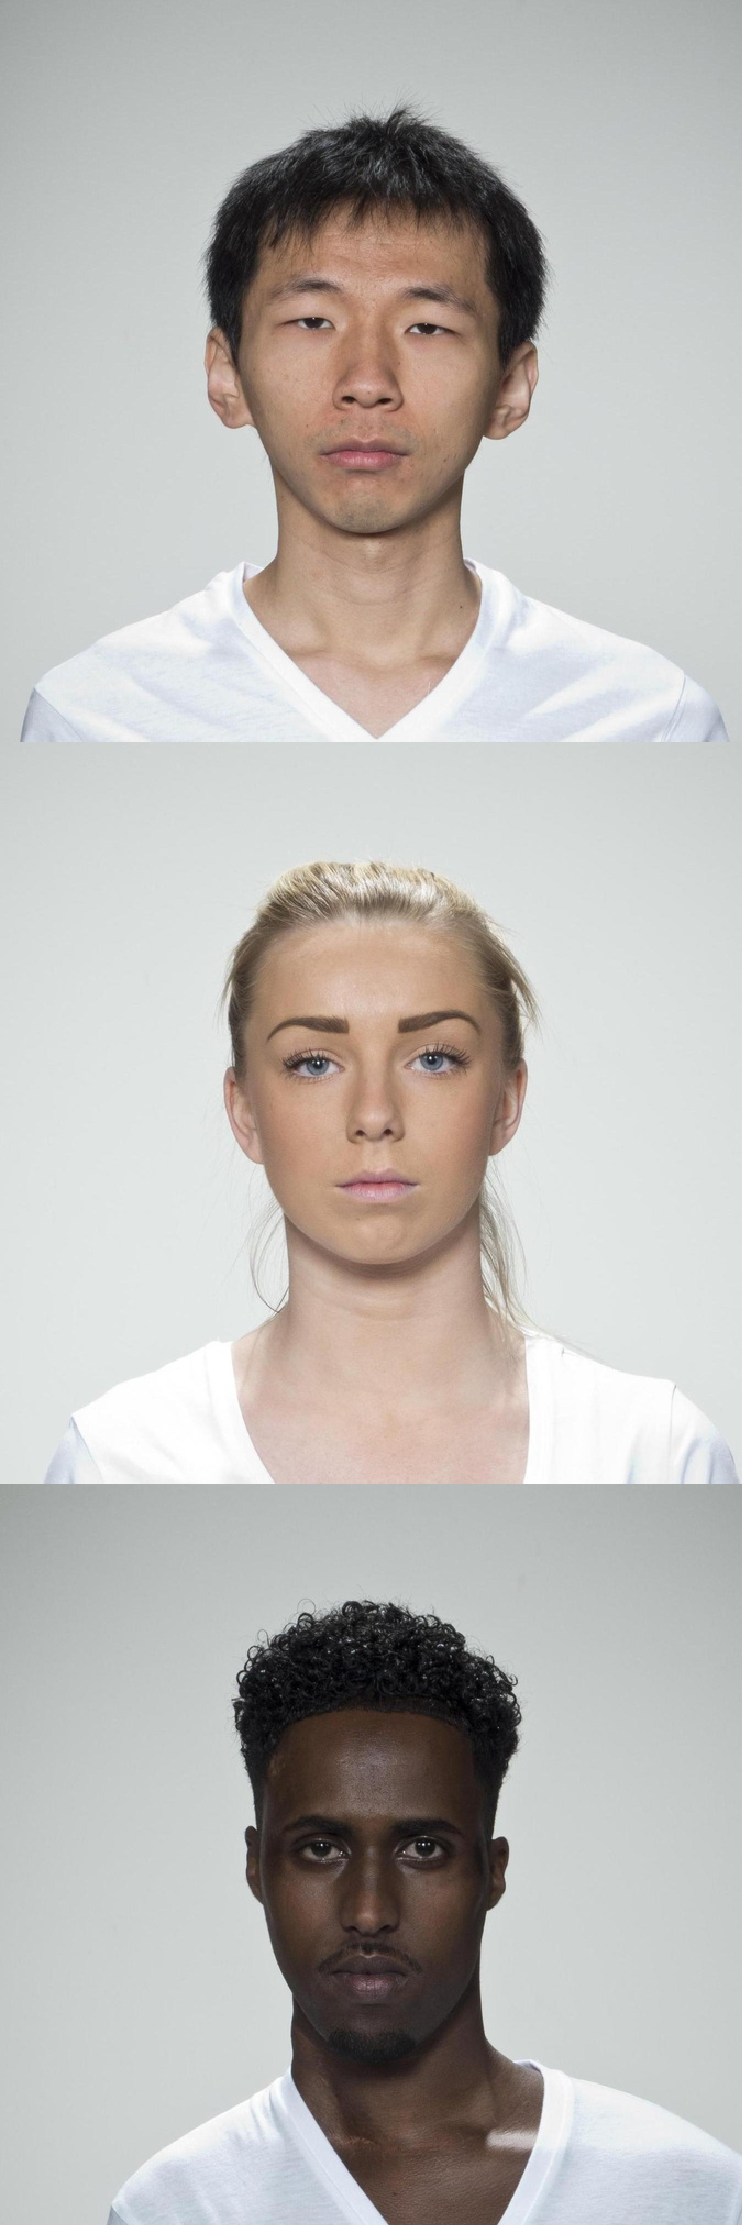
\includegraphics[width=\textwidth]{images/mos_test_set.pdf}\\
        \textbf{(b)} MOS test set % chktex 10
    \end{minipage}
    \caption{Reference images from the MOS set, comprising the selected subjects from the FRLL dataset.}\label{fig:mos_set}
\end{figure}

The printer-proof steganography methods used were based on Generative Adversarial Networks (GANs)~\cite{gans2018} to encode and decode information, illustrated in Fig.~\ref{fig:steganography}, we can obtain various results depending on the method used:

\begin{itemize}
    \item StegaStamp~\cite{stegastamp2020}: claims to be the first steganography model capable of decoding data from printed images. The authors show robust results in decoding data under physical transmission by adding printer noise in the training process.
    \item Code\,Face~\cite{codeface2021}: encoder and decoder networks are trained using end-to-end GANs. It introduces a new security system for encoding and decoding facial images that are printed in common IDs and MRTDs.
    \item RiemStega~\cite{cruz2025riemstega}: proposes a new loss function that extends the loss function based on the $L_2$ distance between images to the Riemannian manifold of symmetric and positive definite matrices.
    \item StampOne~\cite{stampone2024}: focuses on high-level robust steganography, such as~\cite{codeface2021, stegastamp2020}, it balances between high-quality encoded images and decoding accuracy. It mitigates distortion-related issues like JPEG compression, camera sensors and printer's Gaussian noise by incorporating gradient transform and wavelet transform to normalize and balance frequencies of the inputs. 
\end{itemize}

\begin{figure}[ht]
    \centering
    \begin{minipage}[t]{0.2\textwidth}
        \centering
        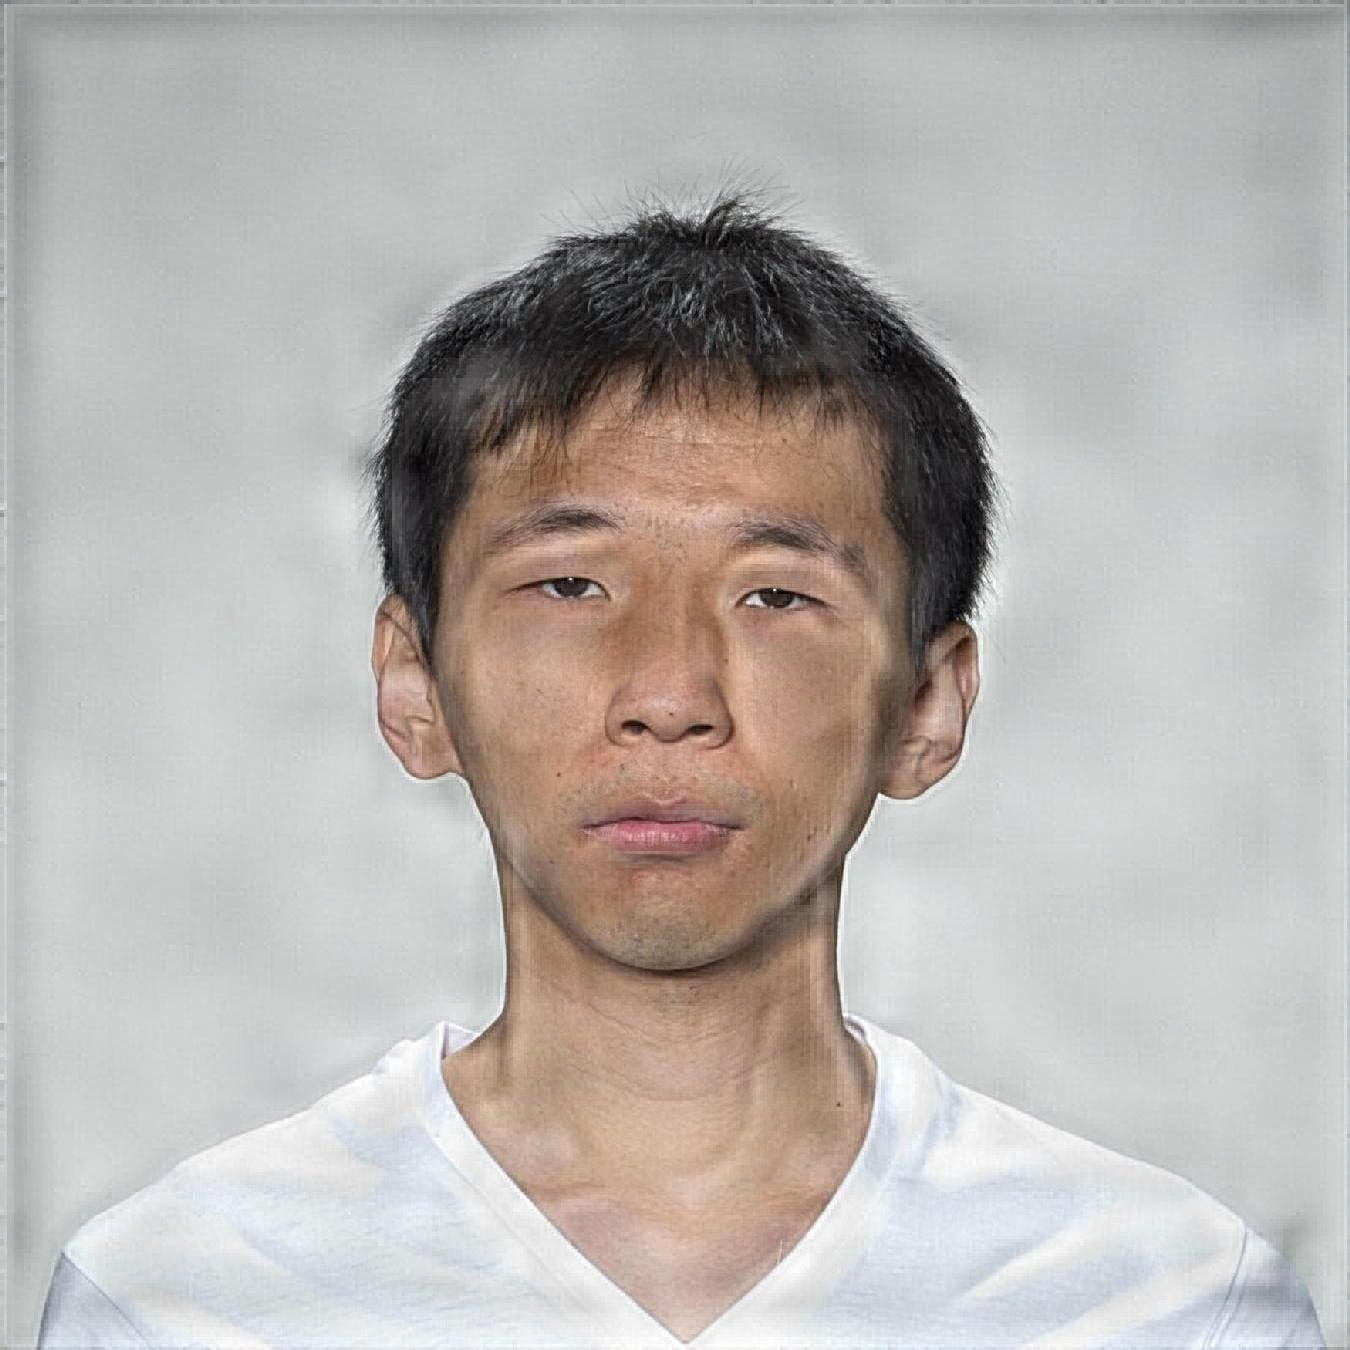
\includegraphics[width=\textwidth]{images/005_StegaStamp_1.4.jpg}\\
        \textbf{(a)} StegaStamp
    \end{minipage}
    \hfill
    \begin{minipage}[t]{0.2\textwidth}
        \centering
        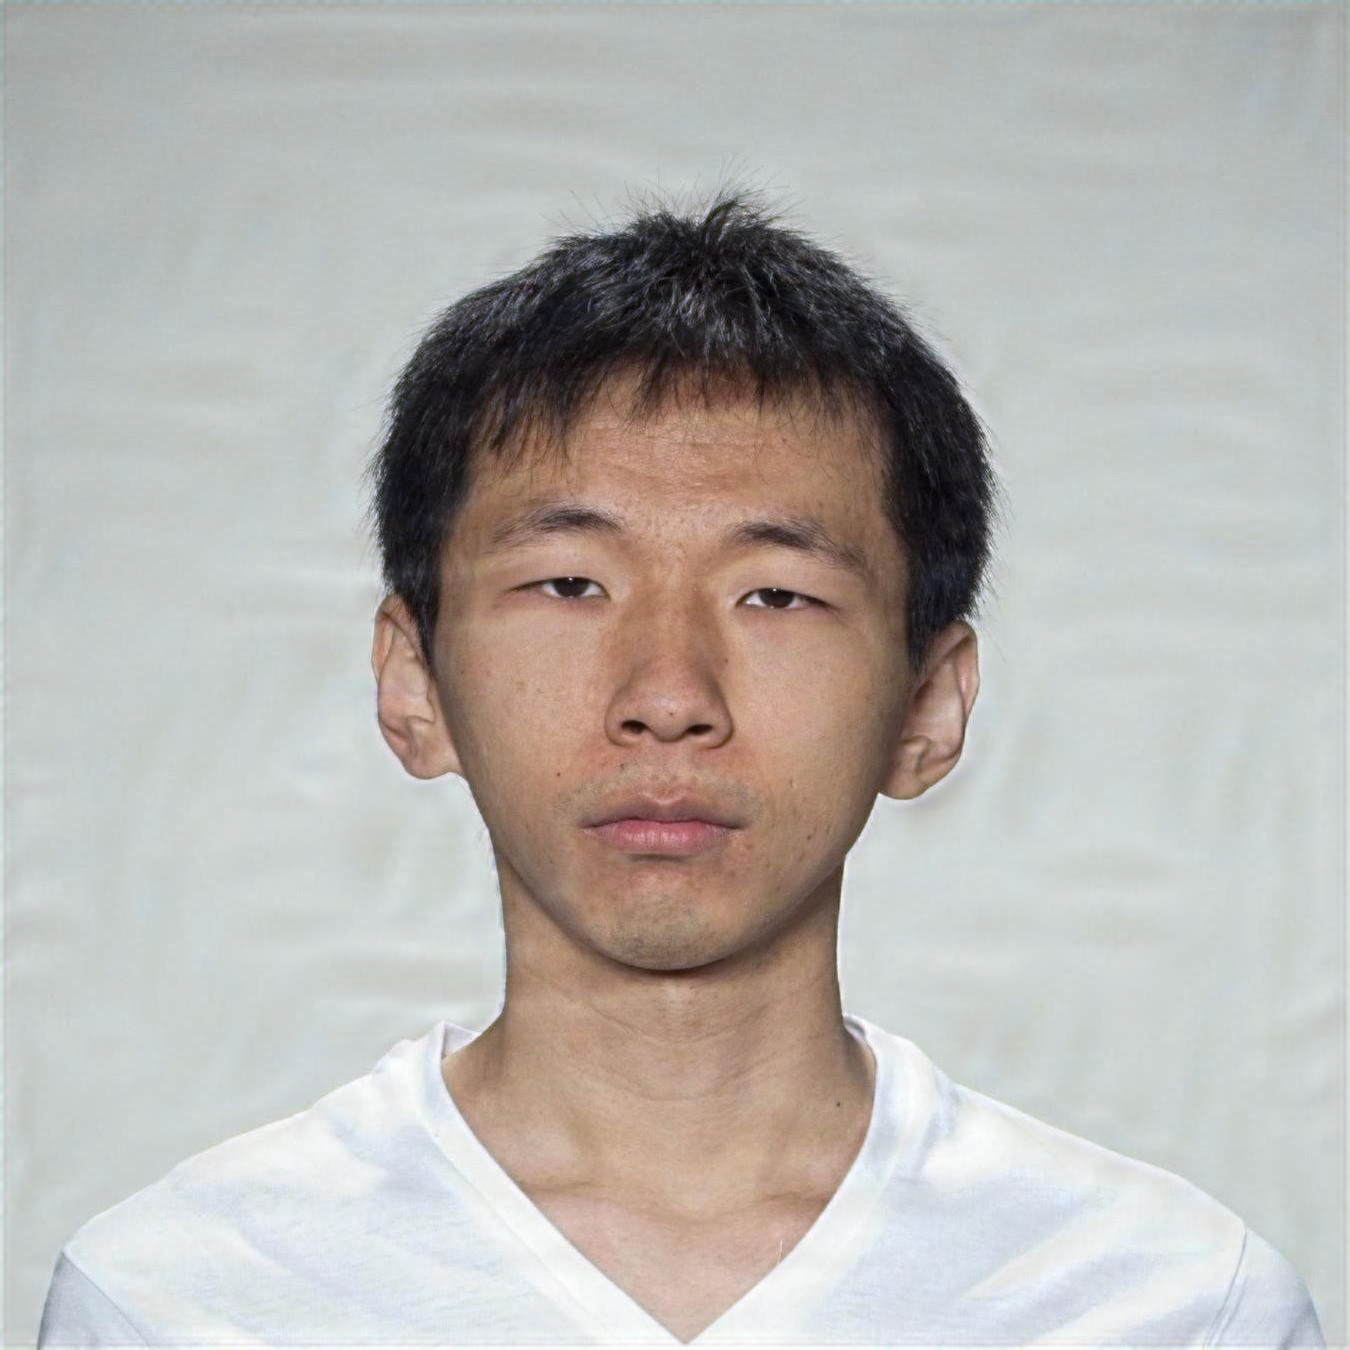
\includegraphics[width=\textwidth]{images/005_CodeFace_1.4.jpg}\\
        \textbf{(b)} Code\,Face
    \end{minipage}
    \hfill
    \begin{minipage}[t]{0.2\textwidth}
        \centering
        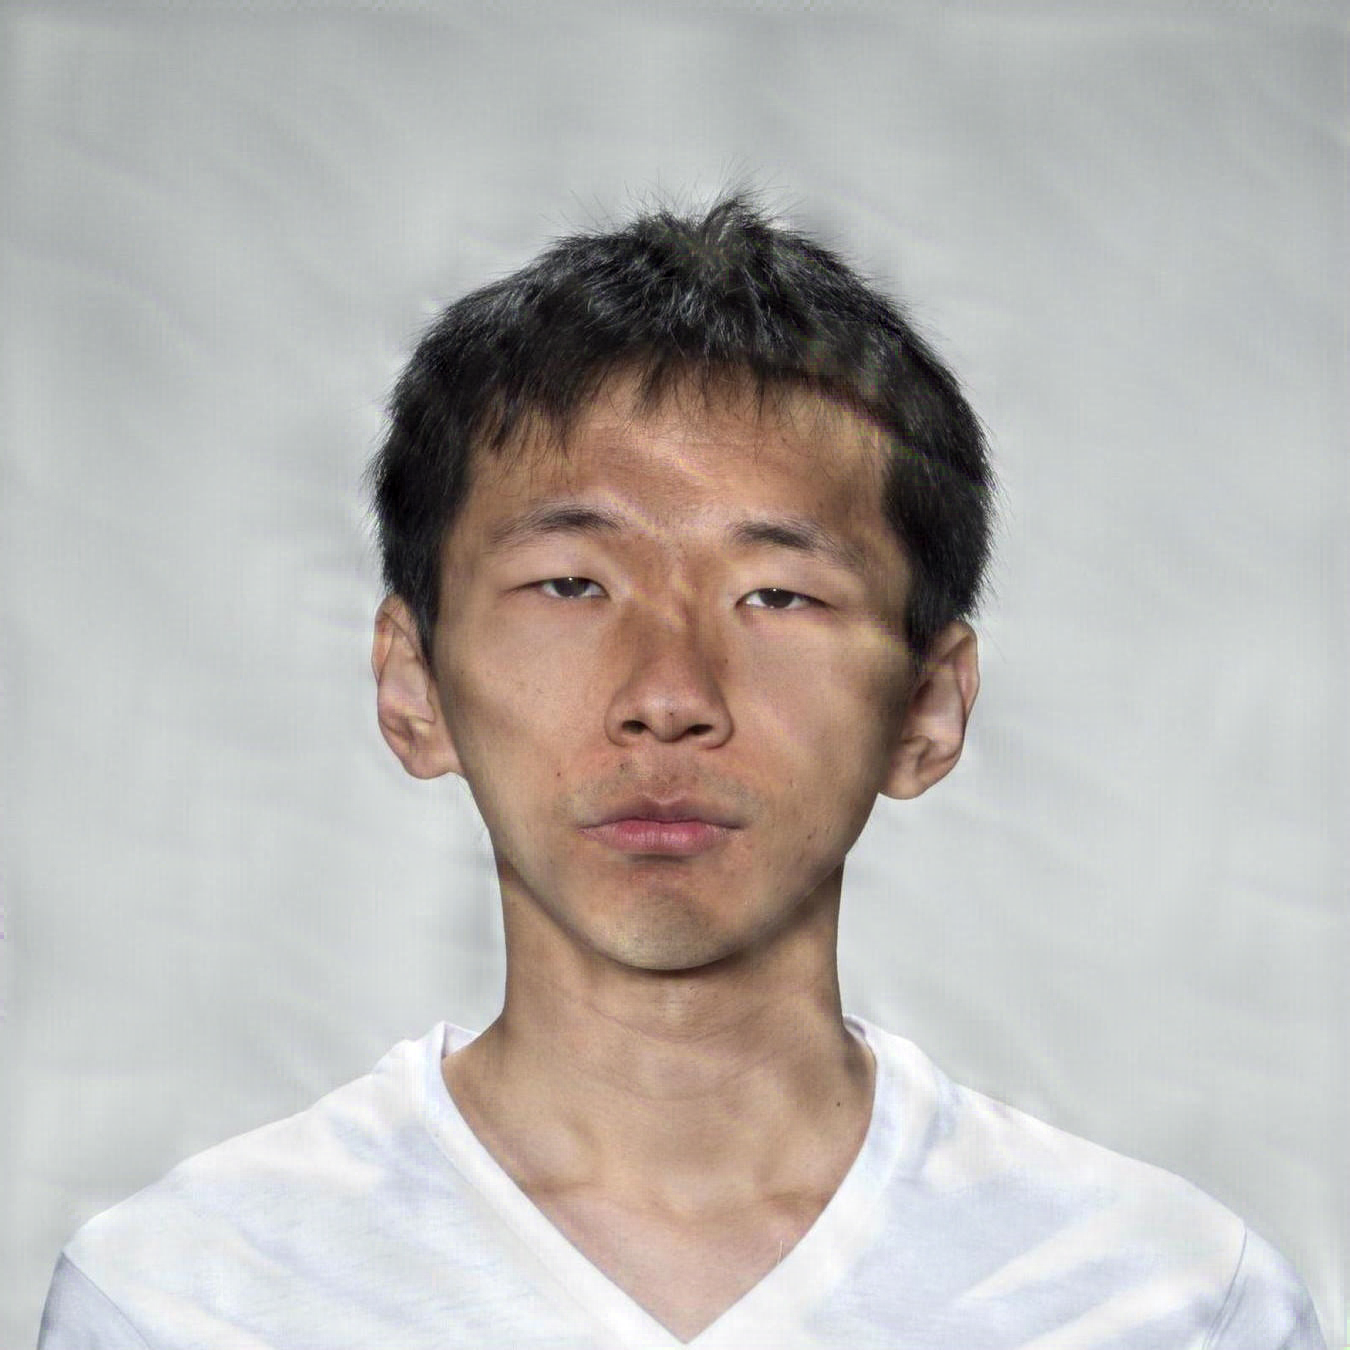
\includegraphics[width=\textwidth]{images/005_RiemStega_1.4.jpg}\\
        \textbf{(c)} RiemStega
    \end{minipage}
    \hfill
    \begin{minipage}[t]{0.2\textwidth}
        \centering
        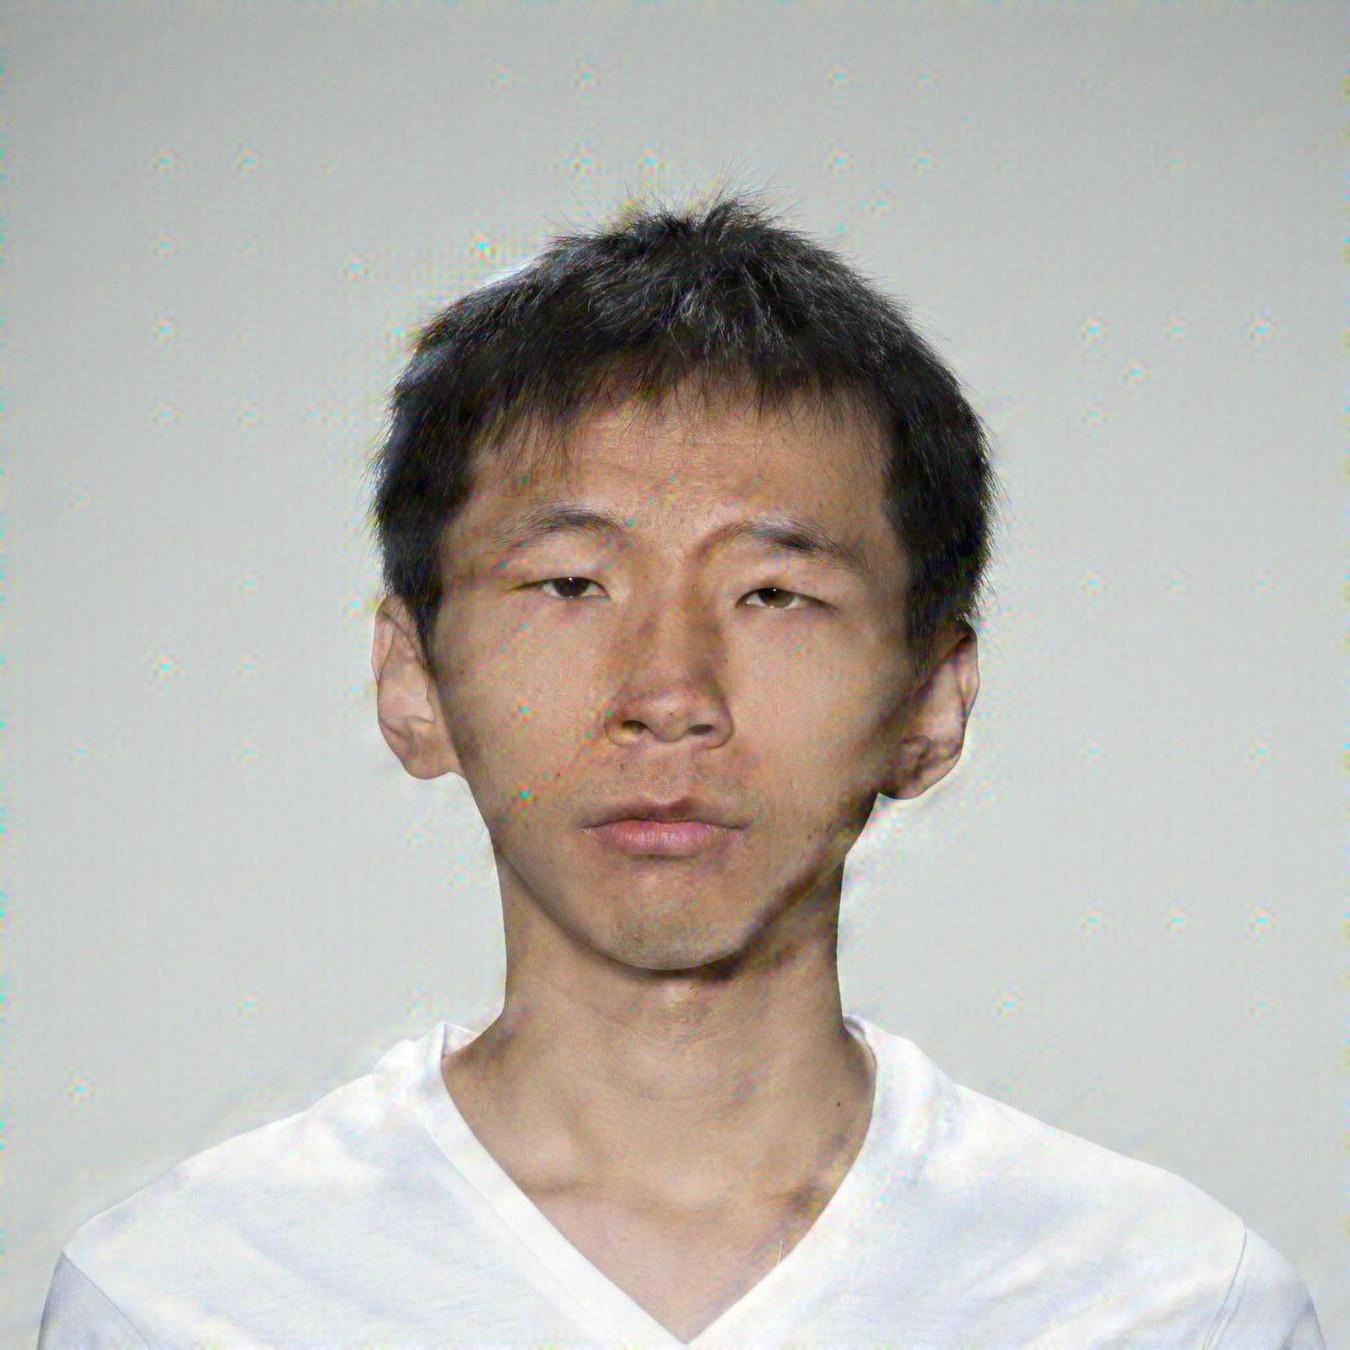
\includegraphics[width=\textwidth]{images/005_StampOne_1.4.jpg}\\
        \textbf{(d)} StampOne
    \end{minipage}
    \caption{Steganographically distorted facial images from each method.}\label{fig:steganography}
\end{figure}


We followed the ITU-R BT.500--15~\cite{ITU-R-BT500} recommendation and adopted the Single Stimulus (SS) method. The test was implemented using a custom Django web application seen in Fig.~\ref{fig:webapp}. Prior to the test session, participants signed an informed consent form and filled out a registration form providing demographic and environmental information such as age, gender, education, country of origin and ethnicity, and others. Each image was shown individually, with no time limit. Ratings were submitted using a labeled slider, and automatic saving ensured session robustness.

Each image in the MOS set was evaluated approximately 30 times by human observers, resulting in over 14,000 ratings. We had around 200 participants, each session lasted about 22 minutes and included roughly 70 evaluations. Following the session, outlier observers were identified and removed using both Kurtosis-based and correlation-based post-screening methods described in ITU-R BT.500--15~\cite{ITU-R-BT500}, resulting in the exclusion of four participants.

\begin{figure}
    \centering
    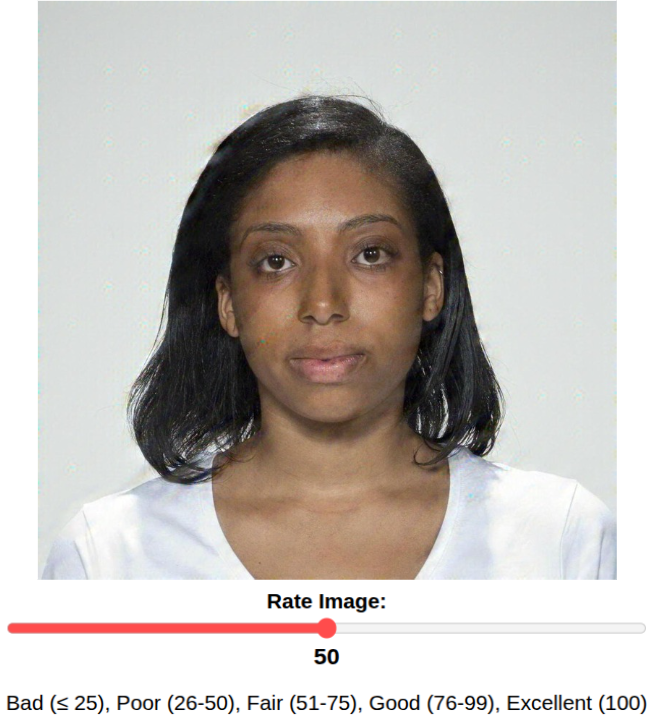
\includegraphics[width=0.32\textwidth]{images/webapp_test.png}
    \caption{Django-based webapp created for the Single Stimulus test.}\label{fig:webapp}
\end{figure}

\subsection{Debiasing of Subjective Scores}

To correct for demographic bias in the subjective scores, we followed a procedure inspired by prior work on bias correction in perceptual tasks~\cite{clapes2018apparent}, where we applied a residualization method based on linear modeling. An ordinary least squares (OLS) regression was fit to the MOS values, using observer and image attributes, and their pairwise interactions as categorical predictors. The fitted bias components were subtracted from the original scores, and the residuals were mean-centered to preserve the global score distribution. As shown in Table~\ref{tab:anova}, several factors exhibit statistically significant effects on the MOS prior to residualization, notably observer and subject ethnicity. After applying the residualization procedure, these effects disappear, as confirmed by an ANOVA test showing no significant impact from any individual factor. The corrected MOS labels are then used as ground truth in all supervised stages of the pipeline to ensure fairness and reduce the influence of socially conditioned priors.

\begin{table}
    \centering
    \caption{ANOVA~\cite{ross2017one} results for observer and image attributes. Before debiasing, several factors show statistically significant effects on MOS, p-value $< 0.05$.\@ After residualization, all main effects show no significant impact, confirming the effectiveness of the debiasing procedure.}\label{tab:anova}
    \begin{tabular}{lcc}
        \toprule
        Factor & p-value & p-value (residualized) \\
        \midrule
        Observer gender                             & 0.022                 & 0.9930 \\
        Observer ethnicity                          & $8.44 \times 10^{-4}$ & 1 \\
        Subject gender                              & $1.60 \times 10^{-3}$ & 0.9722 \\
        Subject ethnicity                           & $7.36 \times 10^{-3}$ & 1 \\
        Observer gender $\times$ Subject gender     & 0.6417              & 0.6417 \\
        Observer ethnicity $\times$ Subject ethnicity & 0.0582              & 0.0582 \\
        \bottomrule
    \end{tabular}
\end{table}

\subsection{Correlation of FR-IQA Metrics with Human Perception}

We compute 40 FR-IQA scores for each distorted image in the dataset and compare them against the corresponding MOS, as seen in Fig.~\ref{fig:mos_vs_iqa}. Several metrics exhibit strong linear trends with MOS, while others are poorly aligned or even negatively correlated. For a detailed description of these metrics, we refer the reader to~\cite{shahrukh2019survey}.



\begin{figure}
    \centering
    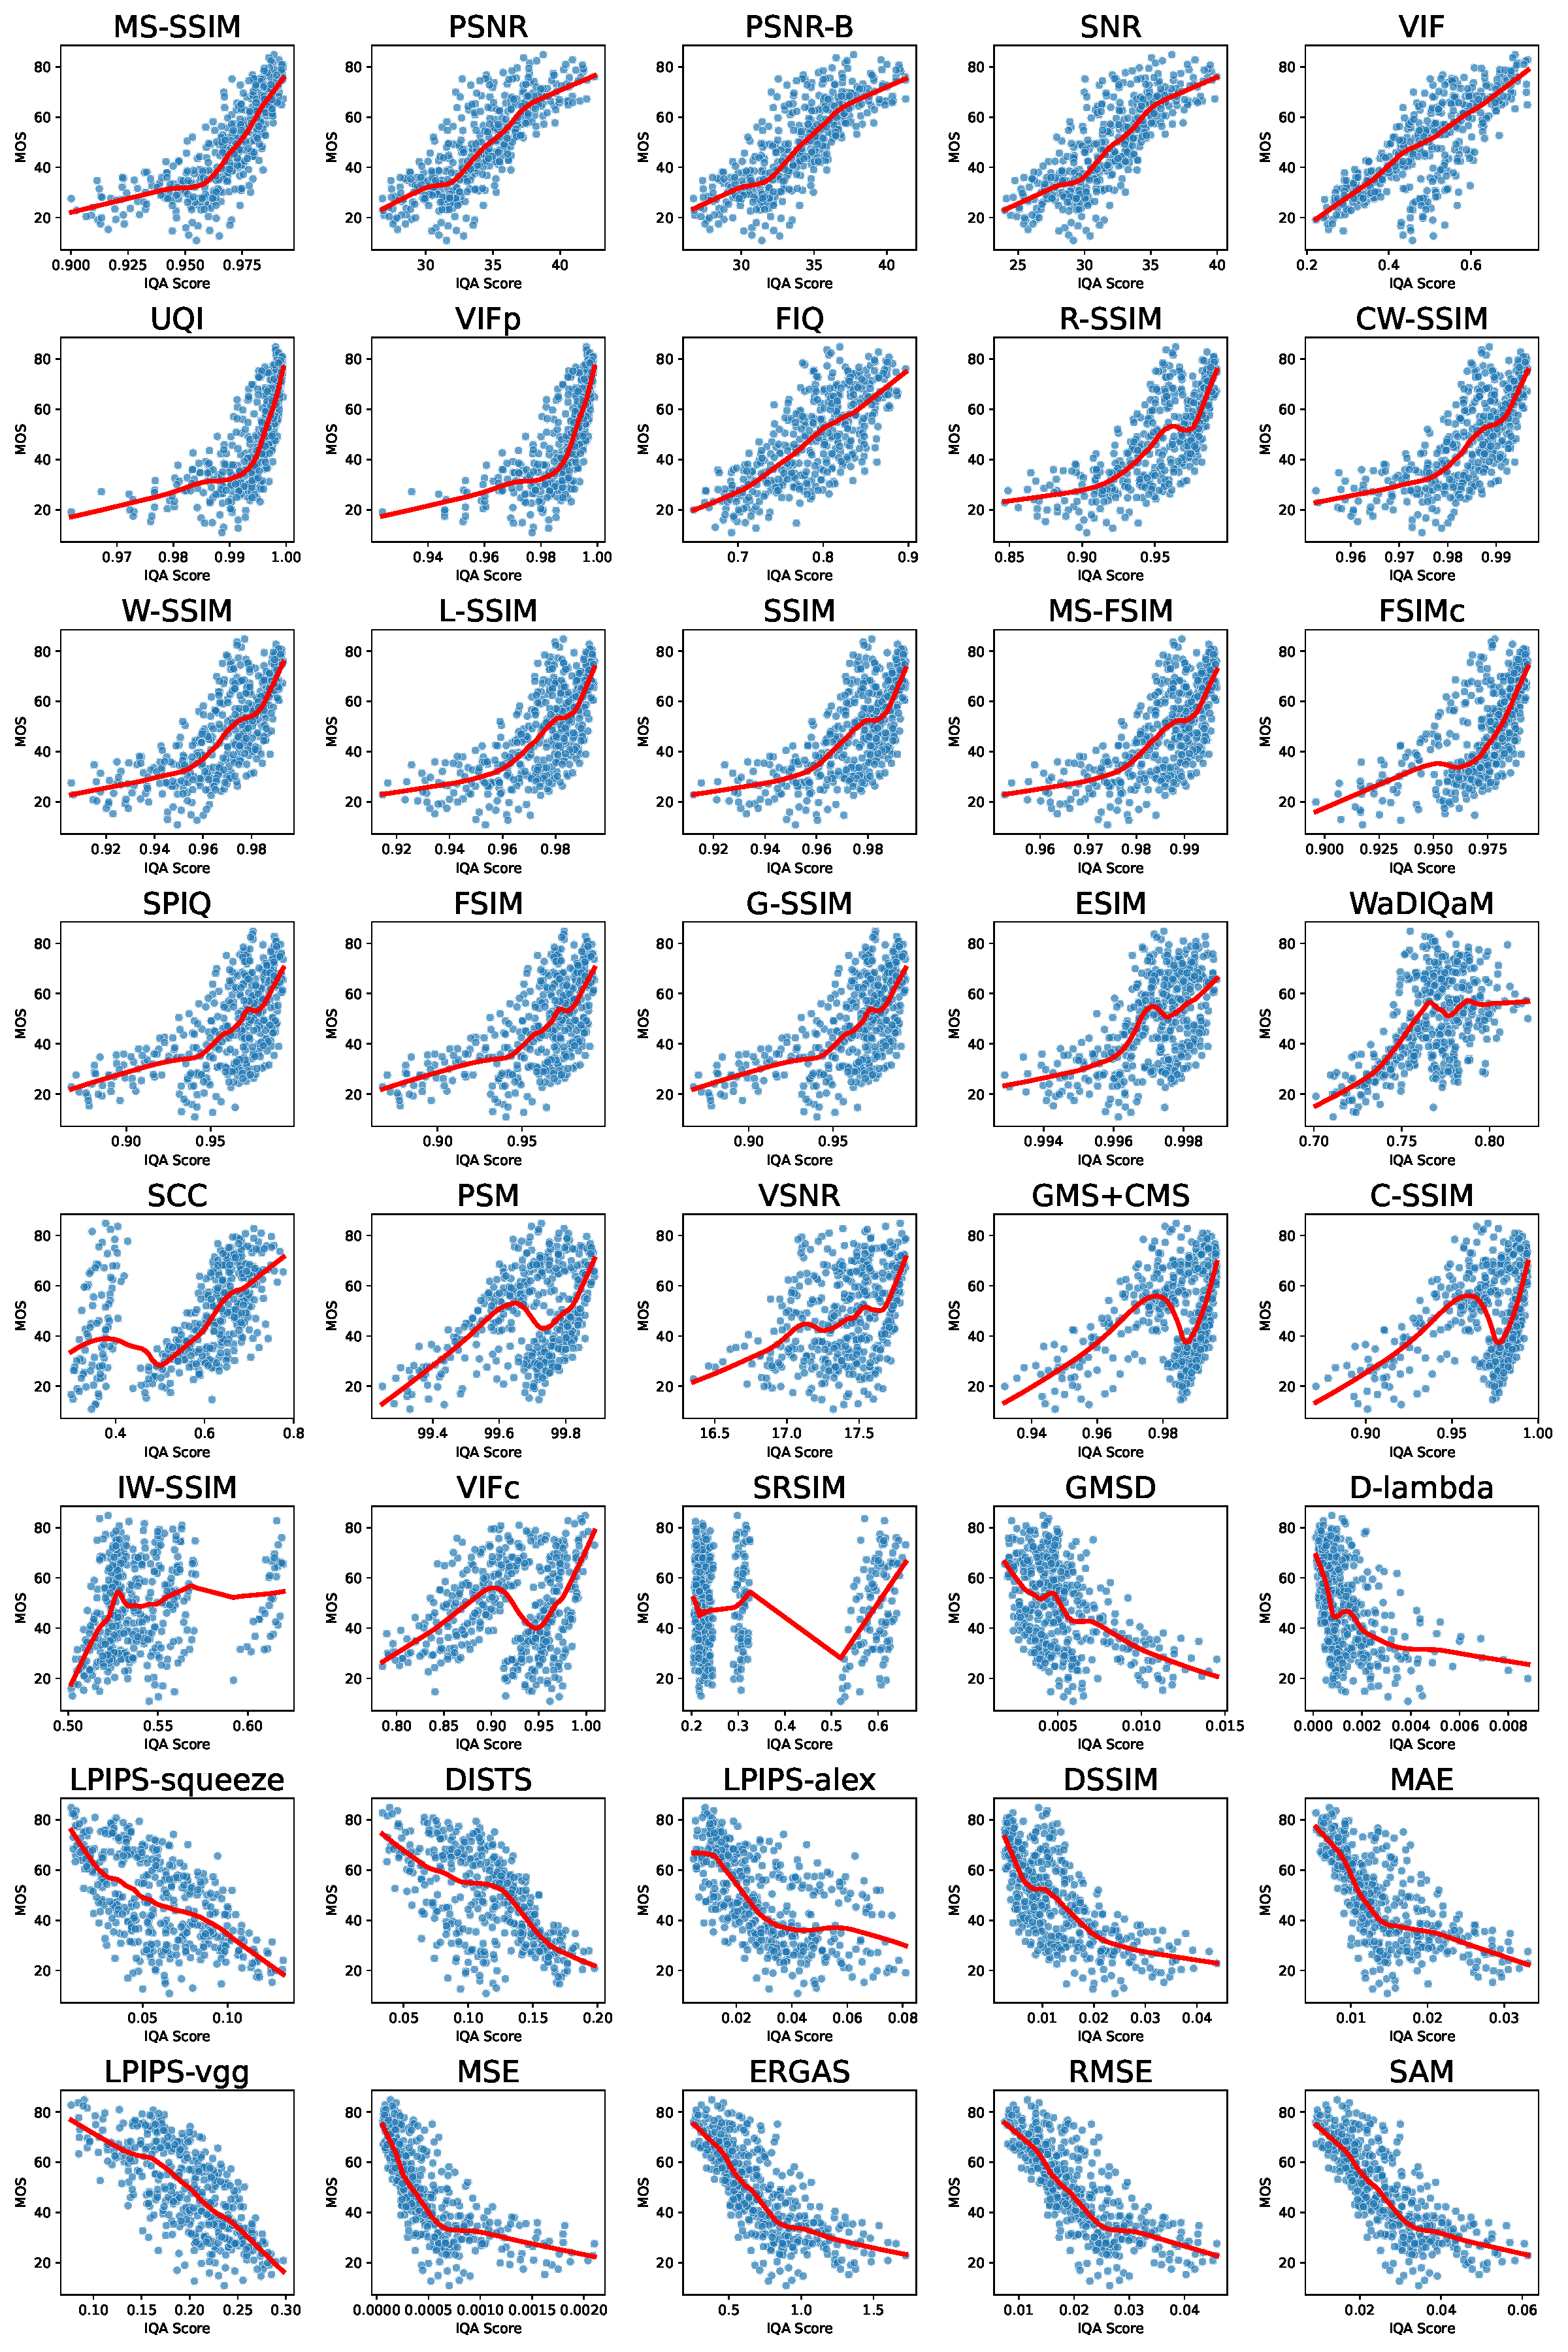
\includegraphics[width=0.98\linewidth]{images/mos_vs_iqa_grid.pdf}
    \caption{Scatter plots illustrating the relationship between MOS and 40 individual full-reference IQA metrics. The red line represents a smoothed local trend curve.}\label{fig:mos_vs_iqa}
\end{figure}

\subsection{Fusion of FR-IQA Metrics for Pseudo-MOS Estimation}

To identify which metrics align best with human perception, we compute both the Pearson Linear Correlation Coefficient (PLCC) and the Spearman Rank-Order Correlation Coefficient (SRCC)~\cite{plcc-srcc} which respectively quantify the linearity and monotonicity of the relationship between metric scores and MOS.\@ To determine the appropriate number of metrics to retain for fusion, we applied Singular Value Decomposition (SVD) and the Picard criterion~\cite{hansen1998picard}. Metrics are first ranked by the average of their PLCC and SRCC with MOS.\@ After normalizing the feature matrix, SVD revealed that six components capture 95\% of the total variance, as shown in Fig.~\ref{fig:svd_analysis}a, indicating an optimal dimensionality of $k=6$.

To validate this truncation point, we examined the Picard plot in Fig.~\ref{fig:svd_analysis}b, which compares singular values with the target projections. The stable ratio in the tail confirms that six components provide a good balance between expressiveness and stability. This supports a compact, informative subset of FR-IQA metrics.

\begin{figure}[ht]
    \centering
    \begin{minipage}[t]{0.48\textwidth}
        \centering
        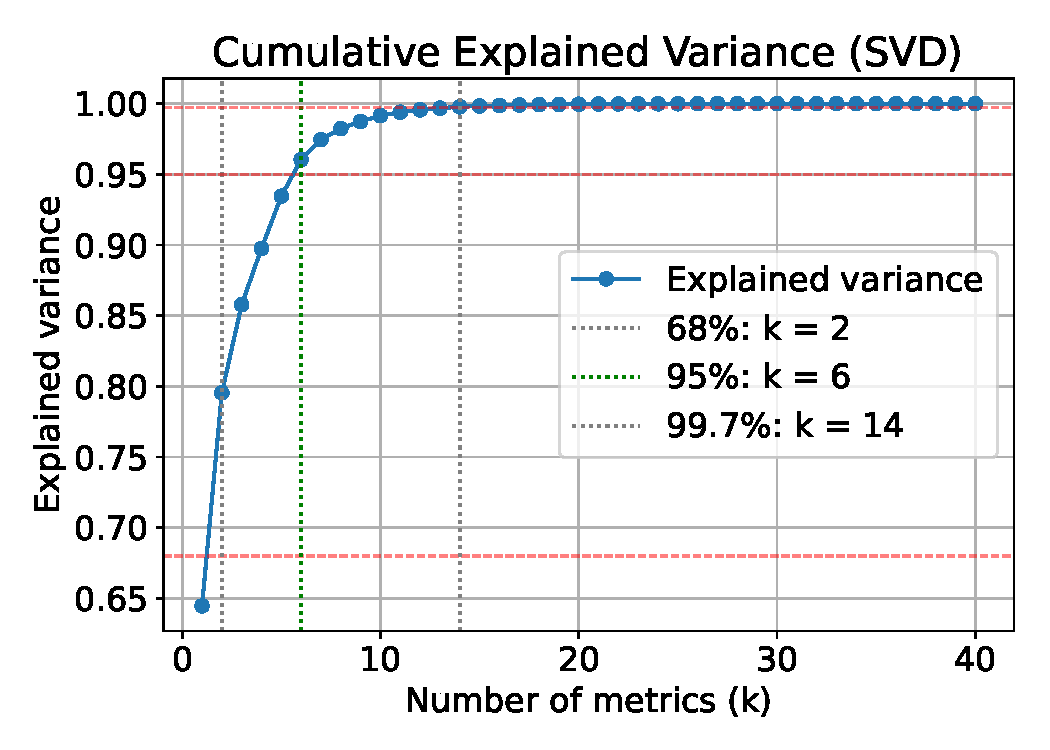
\includegraphics[width=\linewidth]{images/variance.pdf}
        \textbf{(a)} Cumulative variance explained by SVD components.
    \end{minipage}
    \hfill
    \begin{minipage}[t]{0.48\textwidth}
        \centering
        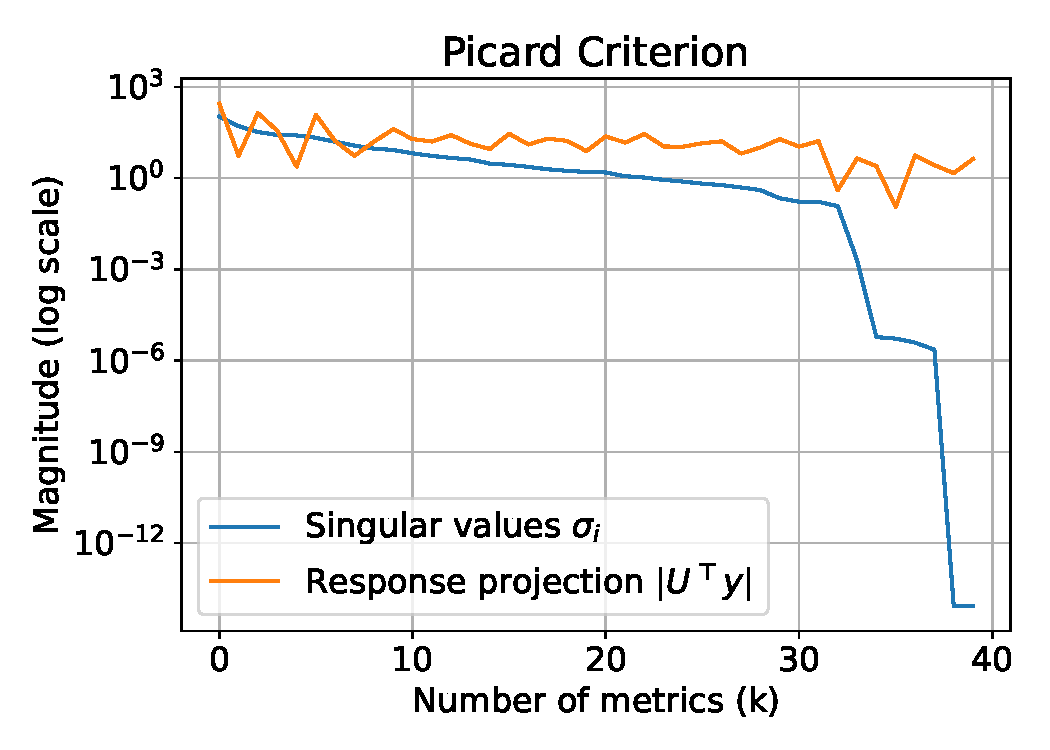
\includegraphics[width=\linewidth]{images/picard.pdf}
        \textbf{(b)} Magnitude of singular values and projected response.
    \end{minipage}
    \caption{SVD-based analysis of the FR metric space. The cumulative explained variance (a) guides the choice of dimensionality, while the Picard criterion (b) illustrates stability near $k=6$.}\label{fig:svd_analysis}
\end{figure}

After selecting the top $k = 6$ FR-IQA metrics, we trained a diverse set of supervised regressors to map these features to subjective MOS scores. The models included both linear and non-linear types:

\begin{itemize}
    \item Linear models: Linear Regression~\cite{linearregression}, Ridge Regression~\cite{ridgeregression}, Bayesian Ridge~\cite{bayesianridge}, ElasticNet~\cite{elasticnet}.
    \item Kernel-based: Support Vector Regression~\cite{svr} (SVR).
    \item Ensembles: Random Forest~\cite{randomforest}, Extra Trees~\cite{ensembles}, Gradient Boosting~\cite{gradboosting}, HistGradientBoosting~\cite{histboost}.
    \item Boosted Trees: XGBoost\cite{xgboost}, LightGBM~\cite{lightgbm}, CatBoost~\cite{catboost}.
\end{itemize}

Each regressor was trained using five-fold cross-validation with an exhaustive grid search over predefined hyperparameter spaces. The best model, CatBoost, optimal configuration was: depth = 8, iterations = 500, learning rate = 0.05, and $L_2$ regularization = 1. This trained regressor is then applied to the unlabeled portion of the dataset (3,132 distorted images), generating pseudo-MOS.\@

\subsection{Training a No-Reference IQA Model from Pseudo-MOS}

To enable NR quality prediction, we train a deep regression model end-to-end using pseudo-MOS scores as targets. The architecture is based on a ResNet-18 backbone~\cite{resnet} pretrained on ImageNet~\cite{imagenet}, with its final classification layer replaced by a lightweight multi-layer perceptron (MLP) regressor~\cite{bayesianridge}. All layers are fine-tuned during training to learn perceptual quality representations specific to our task. The training set consists of distorted facial images paired with either pseudo-MOS, from the FR fusion, or real MOS labels, when available. The model is optimized using MSE and evaluated on the, disjoint, MOS test set of labeled images. Once trained, the model infers image quality solely from the distorted input, enabling NR assessment aligned with human perception.

